\chapter{Evaluation}\label{ch:evaluation}

Since the dataset has no ground truth, the procedure used to pick the parameter values is not comparable to ground truth-based approaches.
Hence, the evaluation is informal and the methods applied have arisen from regular consultation with experts from the tax office.
Run times of different configurations are measured and compared.
Parameters are chosen with respect to model-specific procedures, such as reachability plots for \ac{optics}.
The models are compared to each other and their composition to the baseline topic analysis model \ac{t2v}.


 % Database
 \section{Database}\label{sec:eval-db}
There is a variety of parameter values to choose from when working with databases and embeddings.
These parameters include similarity metrics and the choice of query types.

 \subsection*{Similarity measurements}\label{subsec:evaluation-sim-measurements}

According to \citeauthor{HfsentTrans2019}, the similarity measurements discussed in \autoref{sec:similarity-measurement} 
obtained roughly the same results in their experiments \cite{HfsentTrans2019}.   

% similarity
As the similarity between vectors is usually calculated using some form of cosine similarity, 
rather than Euclidean distance in literature, cosine is preferred over Euclidean distance. 
Since the models may produce embeddings, which are not normalized, the cosine similarity is used instead of the dot product.
Soft cosine similarity is not used, since it is not available in \databaseName{}.
However, the usage of soft cosine would likely improve the results.

 \subsection*{\databaseName{}}\label{subsec:evaluation-db}
% SQL vs NoSQL
According to \citeauthor{flask_book2018}, \ac{sql} databases are a good choice for efficiently storing structured data.
This is because their paradigm \acs{acid}, i.e. \acl{acid}, provides high reliability.
\ac{nosql} databases, on the other hand, are more flexible and can be used to store unstructured data \cite{flask_book2018}.
They do not require a predefined schema and can therefore accept documents of arbitrary structure \cite{flask2018}.
Usually, \ac{nosql} databases do not offer services such as \texttt{JOIN} \cite{flask2018}.
%According to \citeauthor{flask2018}, \ac{nosql} databases make a tradeoff between storage and speed, as well as a tradeoff between consistency and availability.
\ac{nosql} databases are said to outperform out-of-the-box \ac{sql} databases \cite{flask2018}.
Since the dataset consists of unstructured documents and the task at hand does not require performing any \texttt{JOIN}s a \ac{nosql} database is favourable.
\databaseName{} was chosen since it is well known to provide near real-time search and to operate on big data.
Subsequently, it is a good fit for the underlying dataset.

% separation of initialisation and insertion
The time necessary to perform the steps of filling the \databaseName{} database has been evaluated and improved throughout this work.
The current time measurements are shown in \autoref{fig:time_init_db}.
Portioning the work with the database is beneficial since it is possible to update the embeddings without having to recreate the database.
Moreover, modulizing the initialization and filling of the database facilitates debugging and comparing the models used to create the embeddings.

\begin{figure}[htp] % htp = hier (h), top (t), oder auf einer eigenen Seite (p).
    \centering
    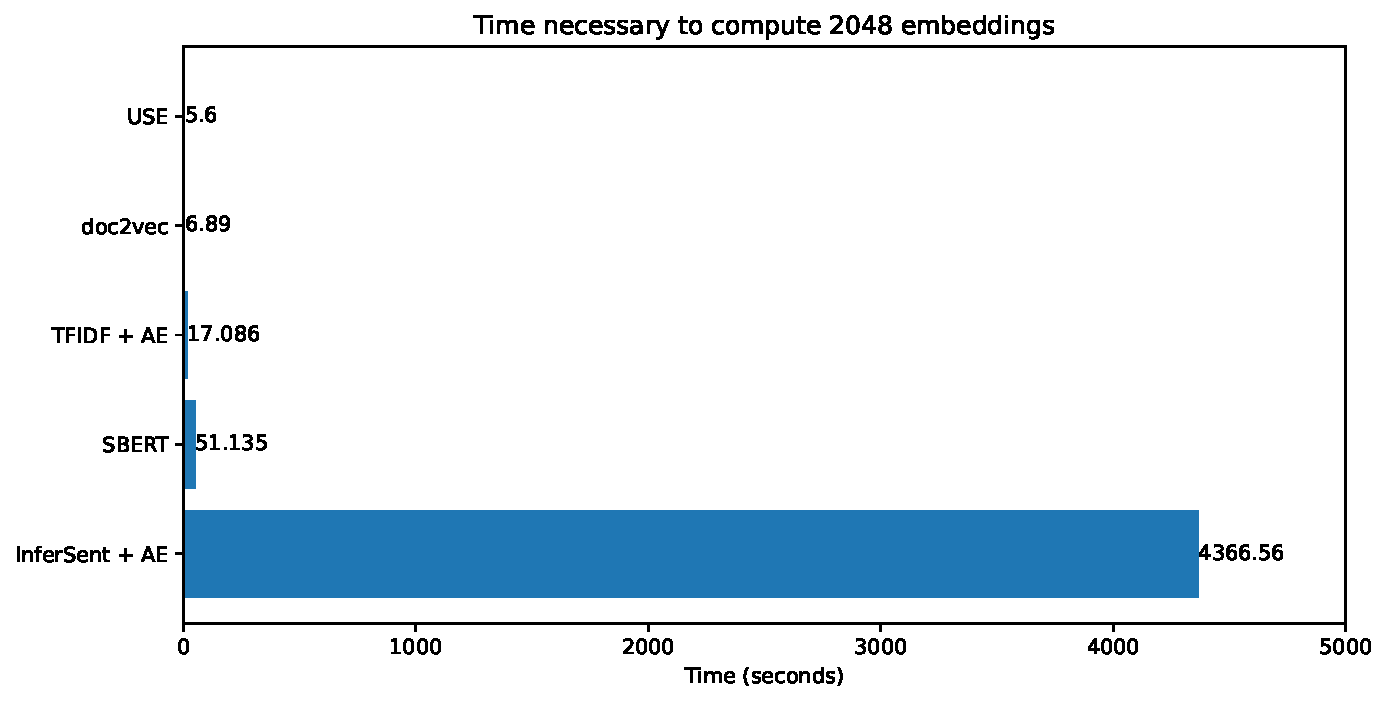
\includegraphics[width=0.6\textwidth]{images/Elasticsearch/Time_necessary_to_compute_2048_embeddings.pdf}
    \caption[Times for creating the database]{Time per module of creating the Bahamas database using a random selection of 2048 documents.
    The reference time was measured using \texttt{cProfiler} on a \localMaschineStats{}.
    %the \texttt{timer} from \texttt{timeit.default\_timer} on a \localMaschineStats{}.
    }
    \label{fig:time_init_db}
\end{figure}

%A document store database can be used if the primary goal is to write fast rather than write save \cite{flask2018}.

 % Eigendocs
 \section{\eigendocs{}}\label{sec:evaluation-eigendocs}
% idea 
% Assuming the layout holds information about the document type, the first page of each document is used to extract this information.
% In the course of working with low-quality versions of the documents to minimize the memory necessary to store them, some documents looked similar.
% Therefore, the idea arose to use clustering algorithms to group the documents according to their appearance.

% number of components
In order to determine the optimal number of components used for \eigendocs{} the cumulative explained variance and the reconstruction error are plotted 
as displayed in \autoref{fig:det_n_comp} from \autoref{subsec:eigenface}.
The first plot indicates that 90\% of the variance is explained by 441 components.
Usually, that would have been the number of dimensions of the subspace onto which the documents would have been projected.
However, when working with clustering algorithms like \ac{optics}, the number of dimensions should be reduced even further to achieve valid clusters.
Therefore the reconstruction error with respect to different numbers of components is taken into consideration.

\begin{listing}[htp]
    \begin{minted}{python3}
        sqr_dif = (X_test - X_test_pca_inverse)**2
        reconstr_err.append(np.sqrt(np.mean(sqr_dif))/
            (np.sum(np.abs(1-X_test))/X_test.shape[0])) 
    \end{minted}
    \caption[Adaption of the \ac{rsme}]{
        Adaption of the \ac{rsme}: 
        Firstly, the squared differences between the original and the reconstructed images are calculated.
        Since the values are normalized, a 1 corresponds to a white pixel.
        Then, the absolute values of all non-white pixels of the test set are summed up.
        The average number of non-white pixels is calculated by dividing the sum by the number of images in the test set.
        This approach considers pixels of value $p \in [0,1]$ as $(p \cdot 100)$\% white and thus, they are incorporated in the sum.
    }
    \label{lst:impl-weighted-rsme}
\end{listing}

Usually, a \ac{rsme} is minimized to determine the optimal parameter configurations.
In this case, the reconstruction error shall be interpreted.
To facilitate the interpretability of the reconstruction error, its calculation is adapted to incorporate the content of the images.
At first sight, the majority of image pixels are white, i.e.\ do not convey any information.
Therefore, the reconstruction error is divided by the average number of non-white pixels. 
Hence, the reconstruction error of an image is weighted by the amount of information it conveys.
The calculation is given in \lst{lst:impl-weighted-rsme}.
The result is displayed in \autoref{fig:det_n_comp}.
Since the reconstruction error increases less rapidly after 10 to 20 components, the number of components is set to 13,
which has been an "elbow" point in a similar trial using a not randomly selected dataset of 195 images.


% results
Some impressions of the \eigendocs{} algorithm are displayed in \autoref{fig:preprocessed_docs_eigendocs}.
Assuming that the selection of documents is representative, 
the preprocessing of the documents using \eigendocs{} should have encoded information about the dimensionality of the images.
However, this assumption is not valid since bigger images exist.
Therefore, the idea of incorporating information about the image's dimensions is not entirely implemented.
 
 % Embeddings
\section{Embeddings}\label{sec:eval-embeddings}
As discussed in \autoref{subsec:impl-embeddings}, there is a range of possible parameter values to choose from when implementing embedding models.
The section below states which findings have led to the parameter values applied in this work.

\subsection*{\acs{tfidf}}\label{subsec:evaluation-tfidf}

The main obstacle to overcome is the high dimensionality of the \ac{tfidf} embeddings.
Hence, the goal of the parameter selection is to find a way to reduce the dimensionality of the vocabulary to 2048 
which is the maximum vector dimensionality of \databaseName{}.
However, the quality of the embeddings should not decline too much.

% parameter selection
The choice of the preprocessor is investigated with regard to the goal of minimizing the vocabulary size.
Both the default and a custom preprocessor are tested on a data corpus of 2048 randomly selected documents concerning the vocabulary (size).
While the default preprocessor had a vocabulary size of 5893, the custom preprocessor had a size of 5585.
The relative difference likely shrinks with a larger data set, 
since the trend is already visible for two different data corpus sizes in \autoref{tab:tfidf-preprocessor-comparison}.
The custom preprocessor is chosen because it had a smaller vocabulary size.
The differences between both vocabularies are visualized in \autoref{fig:differences-vocabularies}.

As stated in \autoref{sec:eval-db}, the \ac{tfidf} embeddings can be problematic 
with regard to the maximal dimensionality of dense vectors stored in \databaseName{}.
Hence, this work has to employ dimensionality reduction techniques to reduce the dimensionality of the embeddings.


% Please add the following required packages to your document preamble:
% \usepackage[table,xcdraw]{xcolor}
% Beamer presentation requires \usepackage{colortbl} instead of \usepackage[table,xcdraw]{xcolor}
\begin{table}[]
    \caption[Comparison of the default and the custom \ac{tfidf} preprocessor]
    {Comparison of vocabulary sizes resulting from the default and the custom \ac{tfidf} preprocessor on different data corpus sizes.}
    \begin{tabular}{|p{0.55\textwidth}|p{0.2\textwidth}|p{0.2\textwidth}|}
    \hline
                                                                                                    & \cellcolor[HTML]{C0C0C0}{\color[HTML]{000000} \textbf{first trial}} & \cellcolor[HTML]{C0C0C0}{\color[HTML]{000000} \textbf{second trial}} \\ \hline
    \cellcolor[HTML]{C0C0C0}{\color[HTML]{000000} \textbf{document corpus size M}}                 & {\color[HTML]{000000} 195}                                          & {\color[HTML]{000000} 2048}                                          \\ \hline
    \cellcolor[HTML]{C0C0C0}{\color[HTML]{000000} \textbf{custom preprocessor vocabulary size A}}  & {\color[HTML]{000000} 1521}                                         & {\color[HTML]{000000} 5585}                                          \\ \hline
    \cellcolor[HTML]{C0C0C0}{\color[HTML]{000000} \textbf{default preprocessor vocabulary size B}} & {\color[HTML]{000000} 1641}                                         & {\color[HTML]{000000} 5893}                                          \\ \hline
    \cellcolor[HTML]{C0C0C0}{\color[HTML]{000000} \textbf{(B-A)/M}}                                & {\color[HTML]{000000} 120/195 = 0,6153846154}                       & {\color[HTML]{000000} 308/2048 = 0,150390625}                        \\ \hline
    \end{tabular}
    \label{tab:tfidf-preprocessor-comparison}
\end{table}

\begin{figure}%
    \centering
    \subfloat[\centering The terms only present in the vocabulary produced by the default preprocessor.]{{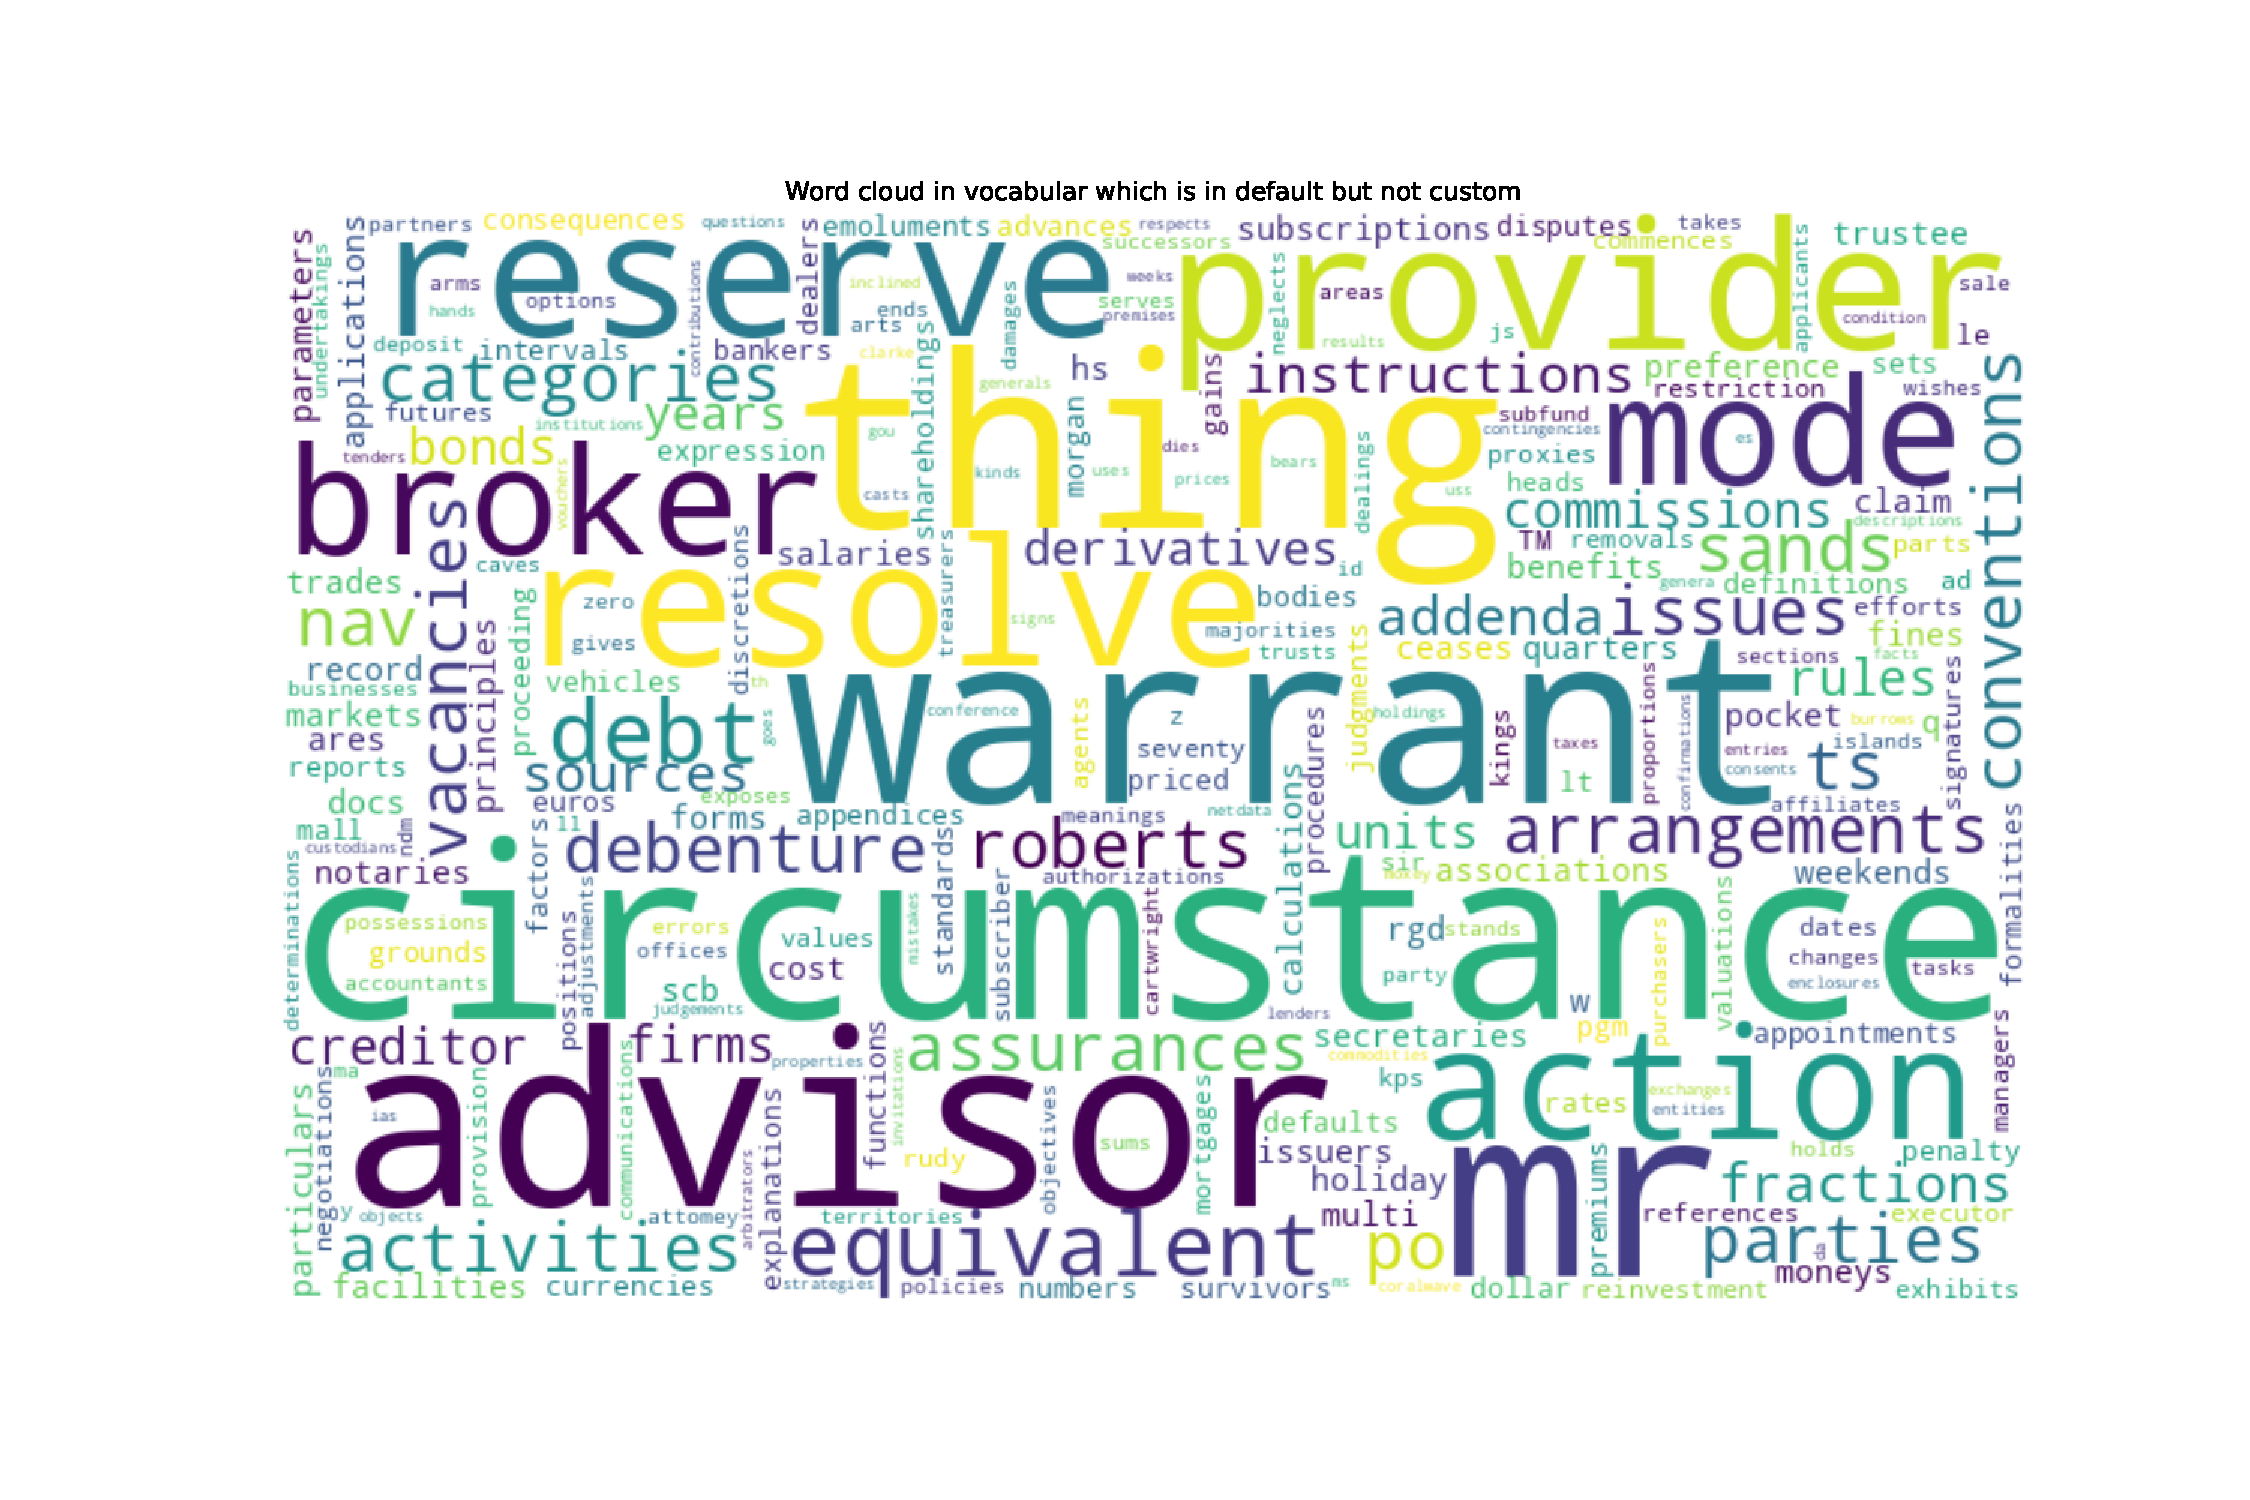
\includegraphics[width=6.8cm]{images/embeddings/tfidf/Word_cloud_in_vocabular_which_is_in_default_but_not_custom.pdf} }}%
    \qquad
    \subfloat[\centering The terms only present in the vocabulary obtained from the custom preprocessor.]{{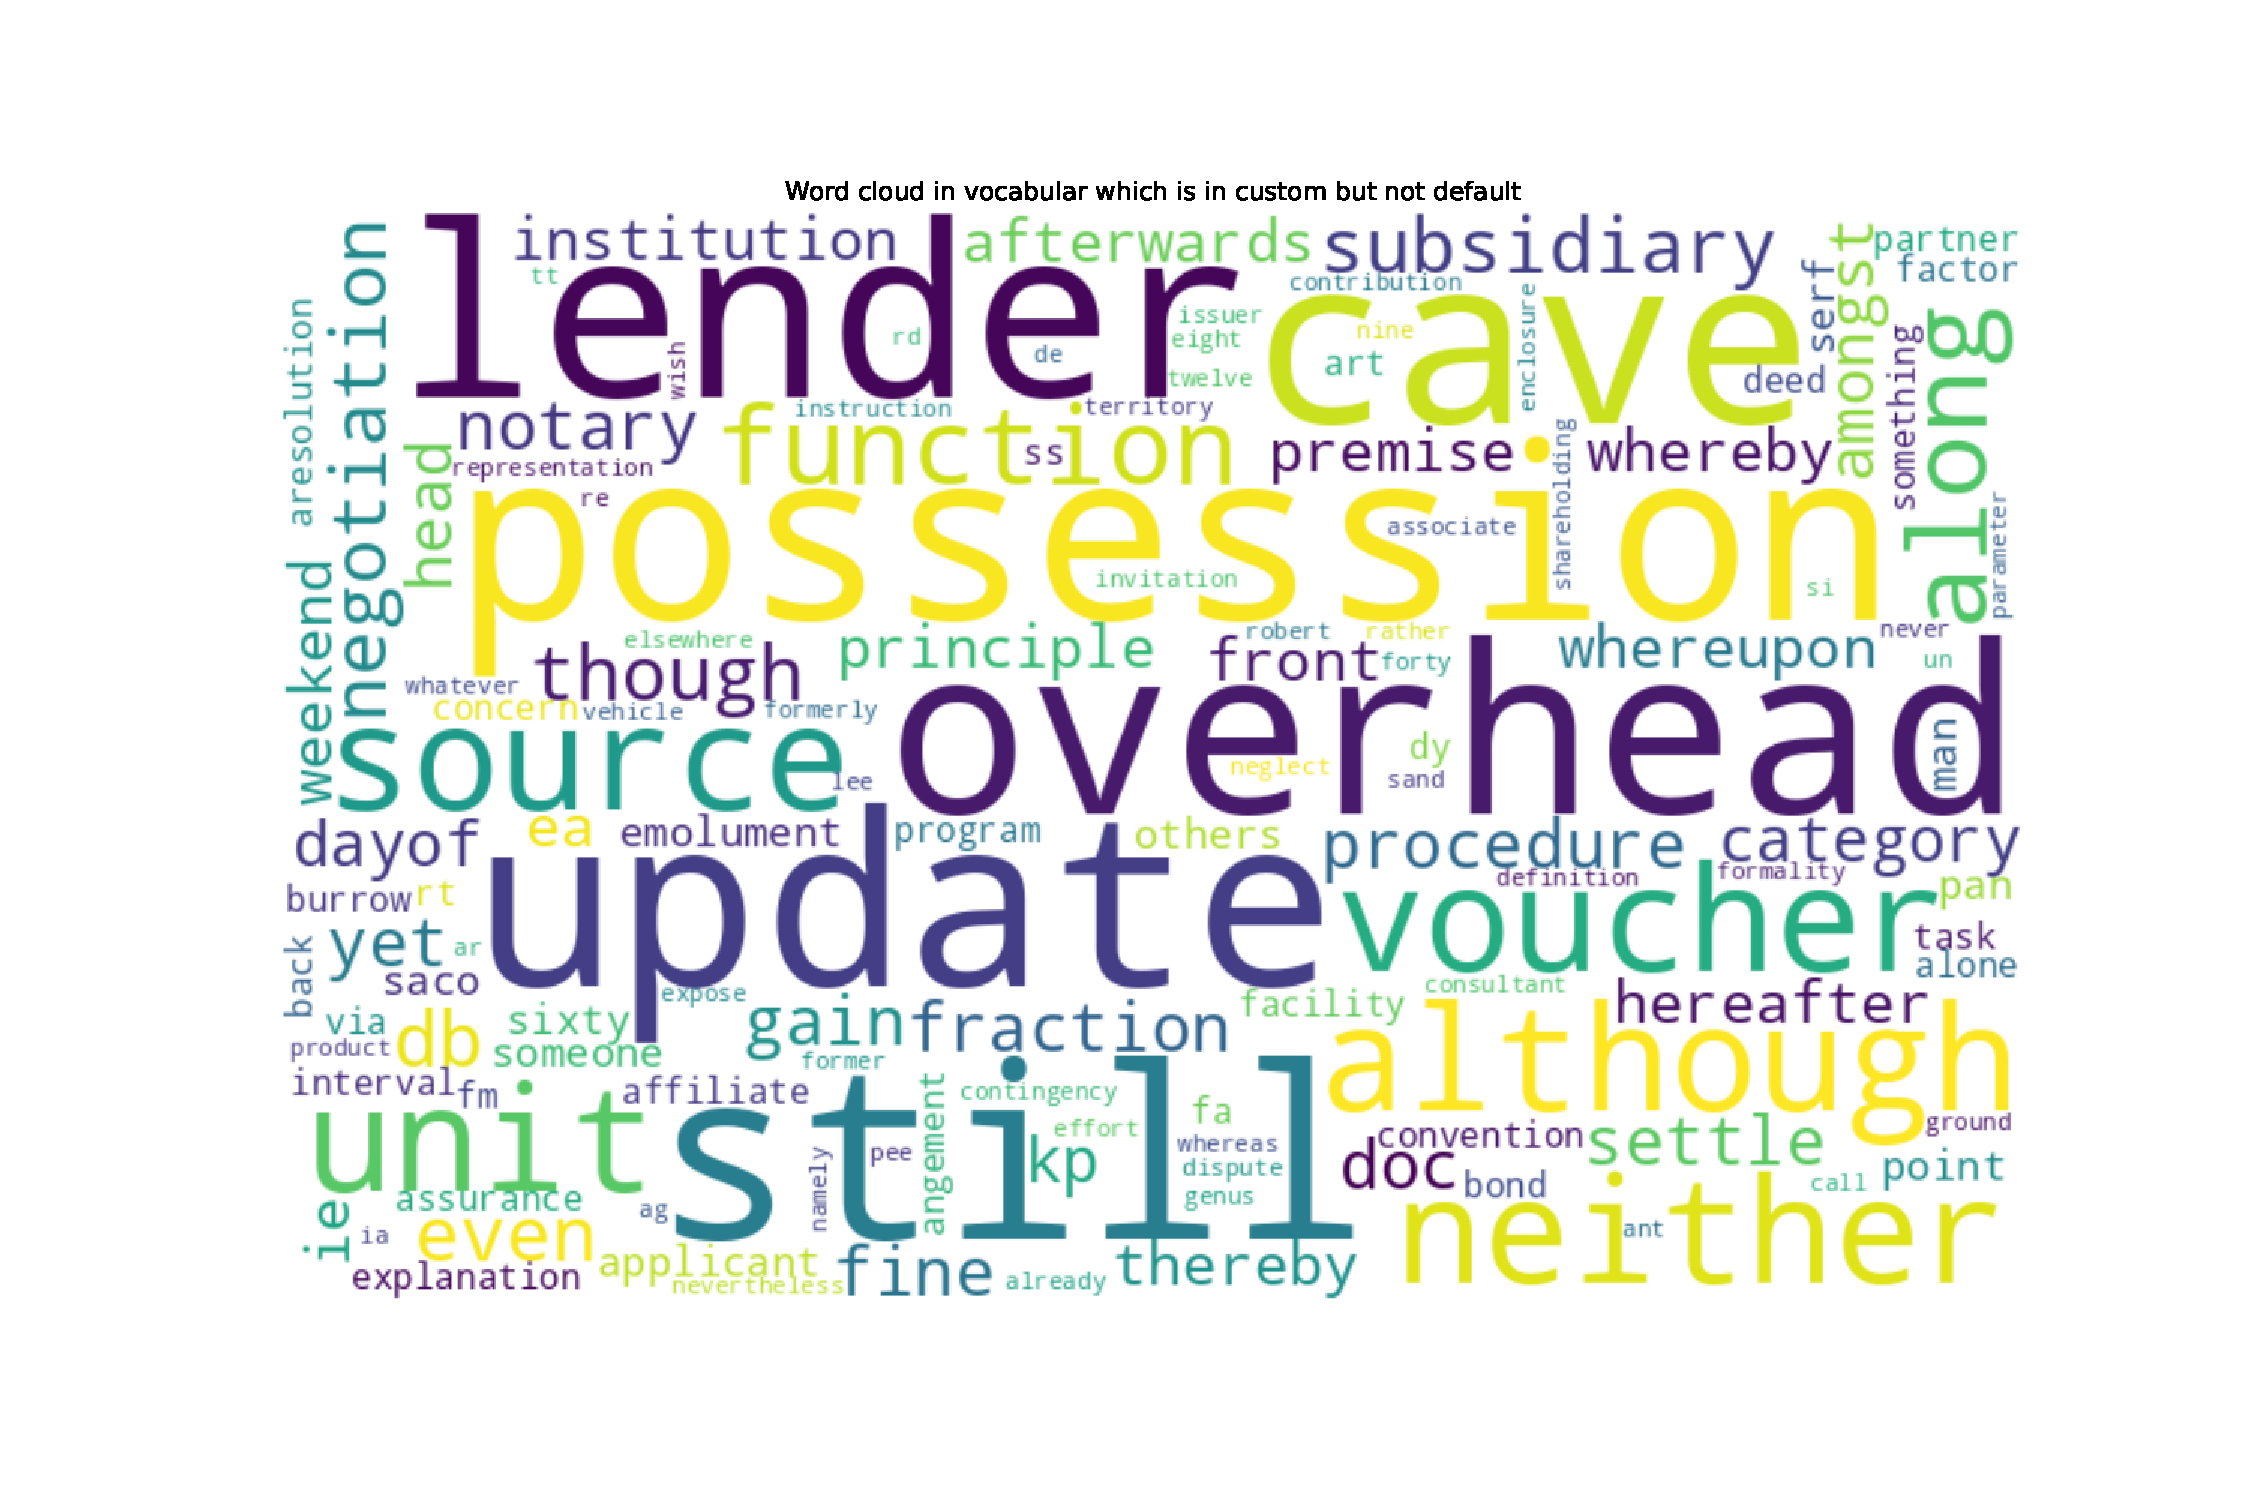
\includegraphics[width=6.8cm]{images/embeddings/tfidf/Word_cloud_in_vocabular_which_is_in_custom_but_not_default.pdf} }}%
    \caption[\wordcloud{}s for different \ac{tfidf} preprocessors]{The \wordcloud{}s visualize which words are unique to both vocabularies 
    on a random selection of 2048 documents.}%
    \label{fig:differences-vocabularies}%
\end{figure}

% two fields in db
Initially, there should have been two different \ac{tfidf} models.
The first one should have been used to obtain documents which are similar to the query document.
Therefore, terms that occur only once in the corpus should have been removed from the vocabulary.
The second approach should have been used to obtain specific documents from the corpus.
Hence, the vocabulary should consist of very document-specific terms and thus, \texttt{max\_df} would have been relatively low, to omit terms that occur in many documents.
However, the restrictions imposed by the database implementation in terms of dimensionality limitations
made it impossible to explore many parameter ranges.
Therefore, only one \ac{tfidf} model is used in the end, whose parameters \texttt{min\_df} and \texttt{max\_df} are set to values 
which kept the vocabulary size small and thus,
the dimensionality of the embeddings is reasonably small.

\subsection*{\ac{d2v}}\label{subsec:evaluation-doc2vec}

Since no labeled data is available, the evaluation of the \ac{d2v} embeddings is limited.
Therefore, the \ac{d2v} embeddings are evaluated by comparing them to other embeddings.
The \ac{d2v} model is not tuned in terms of hyperparameter selection,
but the default settings are used since there is no way to evaluate the resulting embeddings.


\subsection*{\infersent{}}\label{subsec:evaluation-inferSent}

% pool type
The \texttt{max} pooling type is used for the \infersent{} model, since \citeauthor{inferSent2018} 
found by conducting experiments using different pooling techniques that it was the best option.

% version/ embeddings dictionary
Initially, in this work, the \ac{glove} word embeddings were used for the \infersent{} model.
However, since the file of precomputed \acs{glove} word embeddings has a size of 5.65 \ac{gb} and thus,
slows down the model, ultimately another word embedding was used.
The time necessary to compute and insert 195 documents for specific embeddings is displayed in \autoref{fig:times_emb}.
The custom word embedding used in this work is a \ac{w2v} model trained on a selection of 195 documents from the Bahamas dataset.

% glove
\citeauthor{glove2014} state that \acs{glove} outperforms \ac{w2v} on the same corpus, 
vocabulary and window size in terms of quality and speed \cite{glove2014}.
Hence, the quality of the results obtained in this work may have suffered from using a custom \ac{w2v} instead of \acs{glove}.
However, since the computation time of the project is a crucial factor, the custom \ac{w2v} was used.

\begin{figure}%
    \centering
    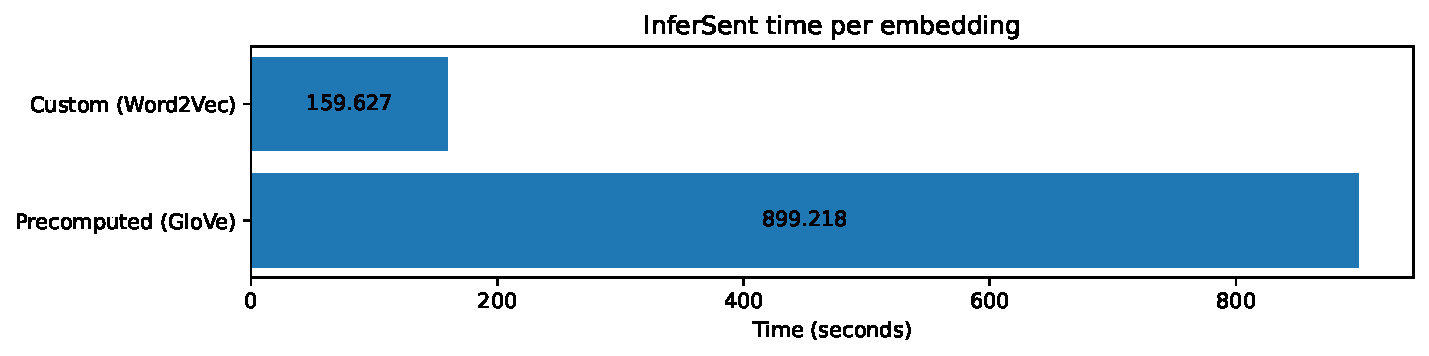
\includegraphics[width=0.6\textwidth]{images/embeddings/infersent/InferSent_time_per_embedding.pdf}
    \caption[Times for \infersent{} embeddings per precomputed word embedding]
    {Time necessary to calculate and insert \infersent{} embeddings for different precomputed word embeddings on a \localMaschineStats{}.
    }
    \label{fig:times_emb}%
\end{figure}


\section{Evaluation of \ac{use}}\label{sec:evaluation-use}

Since there are no parameters to customize the evaluation of the \ac{use} embeddings is limited.
Therefore, the \ac{use} embeddings are evaluated by comparing them to other embeddings.

\subsection*{\ac{ae}}\label{subsec:evaluation-ae}

% architecture
In order to determine, which architecture for the hidden or so-called latent space of the \ac{ae} is the best option, 
different architectures were tested and compared in terms of \ac{rsme} and cosine similarity.
The \ac{rsme} is calculated as given in \lst{lst:impl-rsme}.
The cosine similarity is calculated as given in \lst{lst:impl-cos_sim}.
Due to the fact that cosine similarity values are bound by 0 and 1, they are easier to rank than metrics that can yield any real number.
However, cosine similarity is usually applied to calculate the angle between two vectors and thus, one has to be cautious when interpreting the result obtained.
For instance, the vectors $\left( 0, 1 \right)^T$ and $\left( 0, 2 \right)^T$ have a cosine similarity of 1, even though they are not the same vectors.
Since an \ac{ae} is supposed to reconstruct the input rather than return a dependent or related vector, this metric should be combined with a tarditional metric.
The dataset used for the evaluation is a selection of 195 documents from the Bahamas dataset.

% RSME
\begin{listing}[htp]
    \begin{minted}{python3}
        rsme = np.linalg.norm(inverse_embedding - embeddings) 
                / np.sqrt(embeddings.shape[0])
    \end{minted}
    \caption[Computation of the \ac{rsme}]{
        Computation of the \ac{rsme} between the original and the reconstructed embedding.
    }
    \label{lst:impl-rsme}
\end{listing}

% cosine similarity
\begin{listing}[htp]
    \begin{minted}{python3}
        cos_sim = statistics.mean([np.dot(inverse_emb, embedding)
                /(np.linalg.norm(inverse_emb)*np.linalg.norm(embedding)) 
                for inverse_emb, embedding in zip(inverse_embedding, embeddings)])
    \end{minted}
    \caption[Computation of the cosine similarity]{
        Computation of the cosine similarity between the original and the reconstructed embedding.
    }
    \label{lst:impl-cos_sim}
\end{listing}

The scores of different architectures are shown in \fig{fig:eval-ae-architecture}.
While most of the architectures produced similar results, one architecture stood out.
Combining 2500-, 3000- and 3500-dimensional layers in the hidden space produced the worst \ac{rsme} results.
The best results were achieved by adding a 3500-dimensional layer in the hidden space.
However, the results of the best architecture do not differ greatly from the others.

\begin{figure}[!htb] % htp = hier (h), top (t), oder auf einer eigenen Seite (p).
    \centering
    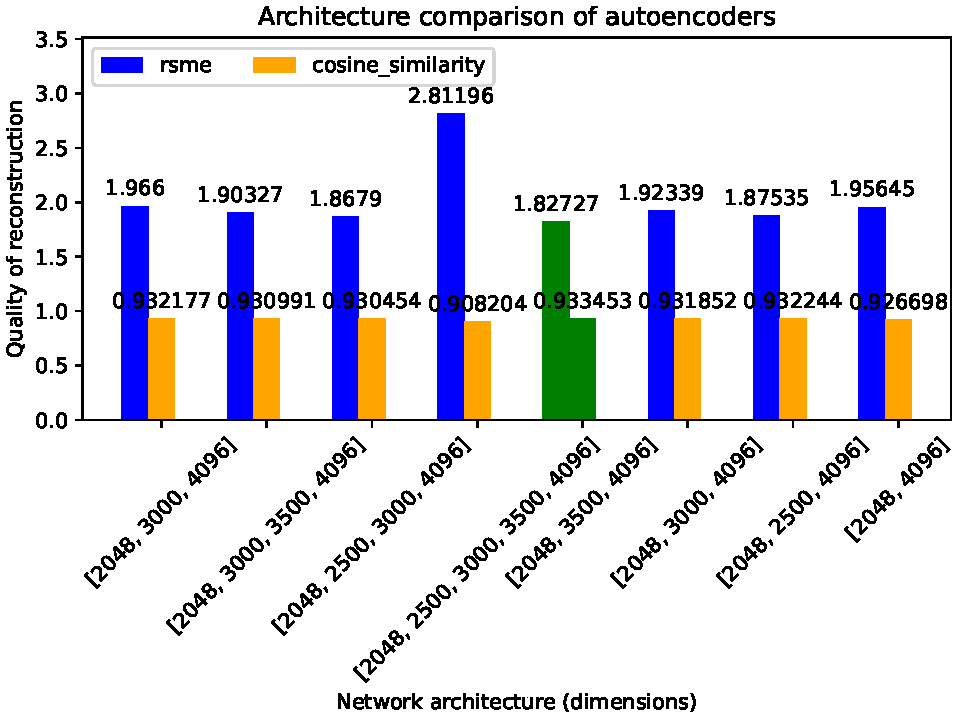
\includegraphics[width=1\textwidth]{images/embeddings/autoencoder/ae_score_plot.pdf}
    \caption[Different \ac{ae} architectures and their reconstruction error]{The effect of different \ac{ae} architectures on the reconstruction error.
    The error is measured in terms of \ac{rsme} (blue bars) and cosine similarity (yellow bars) between the original and the reconstructed image.
    The smallest \ac{rsme} and the biggest cosine similarity belong to the architecture best suited to this task and are coloured green.
    }
    \label{fig:eval-ae-architecture}
\end{figure}

% Clustering
\section{Clustering using \acs{optics}}\label{sec:evaluation-OPTICS}
% 3d plots
The algorithm \ac{optics} was applied to data, which was preprocessed according to \autoref{pt:32} and \autoref{pt:eigendocs}.
The clusters from \autoref{fig:optics_cluster} were extracted from the respective reachability plots in \autoref{fig:reachability_plots}.
The three-dimensional plots visualize the first three dimensions of the data and thus, the weights of the first three principal components assigned by the \eigendocs{} algorithm.
By visual inspection and comparison of both plots, it can be seen that the projection by the combination of resizing and \ac{pca} of \autoref{pt:32} scatters the objects further along the $x_2$ axis.
Hence, the distance between the objects is larger and more clusters are identified.
One could argue that the narrow distribution of the objects in the \eigendocs{} plot is due to the fact, 
that the input data encodes not only the visual appearance in terms of page layout but also the size of the document.
Possibly, this could explain why the objects are less scattered along this dimension.

% OPTIC cluster results
\begin{figure}%
    \centering
    \subfloat[\centering Preprocessing according to \autoref{pt:32}.]{{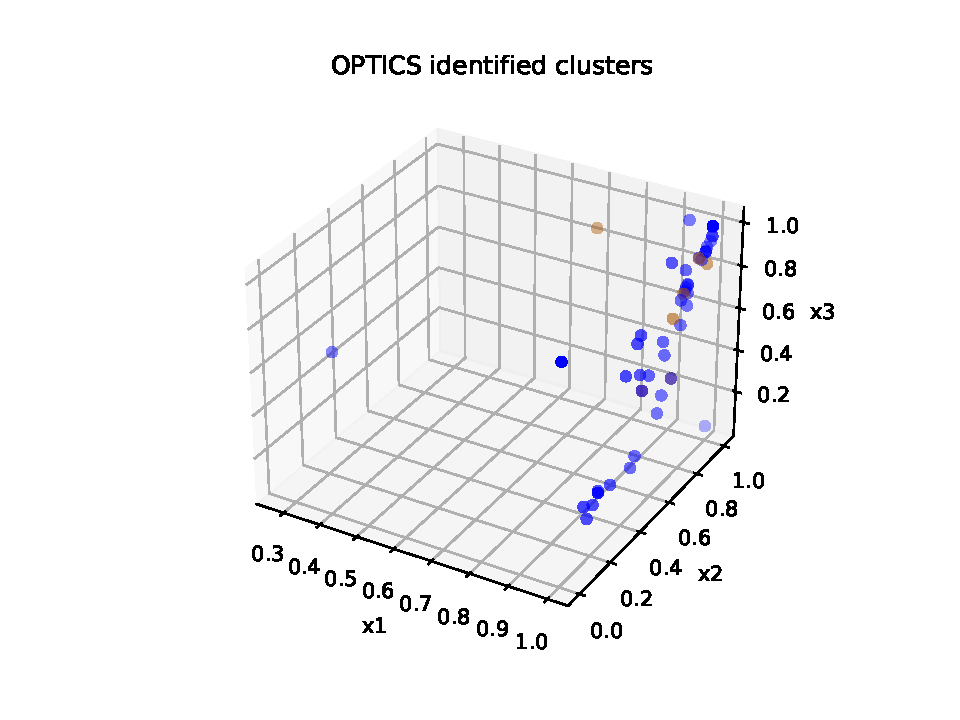
\includegraphics[width=5cm]{images/OPTICS/32x32/OPTICS_cluster_32x32.pdf} }}%
    \qquad
    \subfloat[\centering Preprocessing according to \autoref{pt:eigendocs}.]{{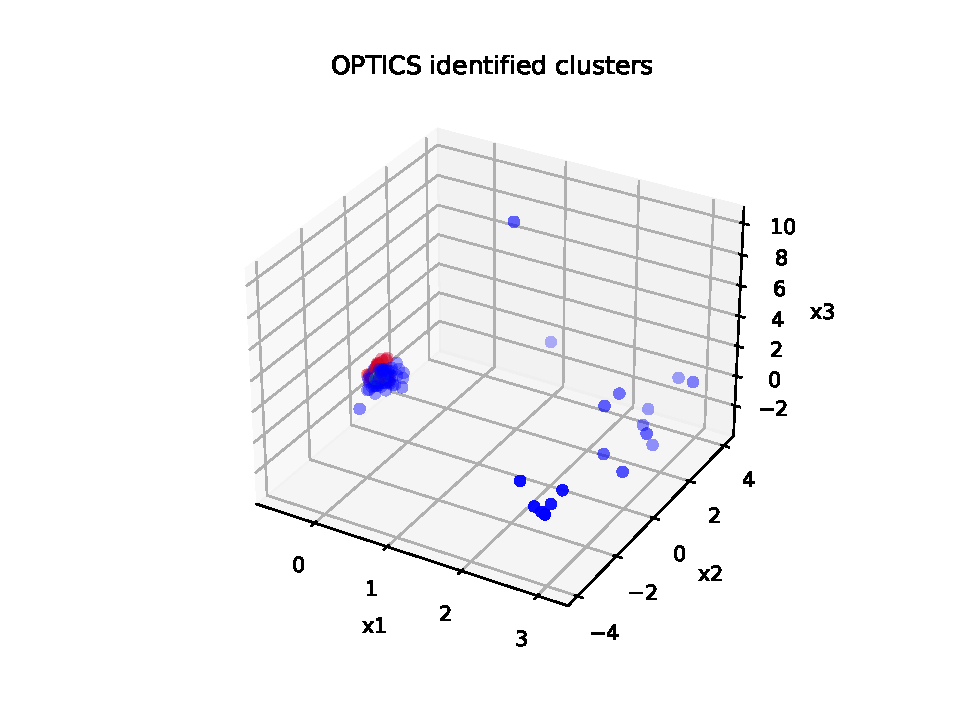
\includegraphics[width=5cm]{images/OPTICS/eigendocs/OPTICS_cluster_eigendocs.pdf} }}%
    \caption[\ac{optics} clusters]{The clusters were extracted from the respective reachability plots in \autoref{fig:reachability_plots} by \ac{optics}.
    The blue points are noise points, whereas any other colour denotes a cluster.}%
    \label{fig:optics_cluster}%
\end{figure}



% cluster content
To analyse the results of the clustering, the content of the clusters was examined.
Since the documents are not labelled, the content of the clusters was analysed by visual inspection.
The content of the clusters is displayed in \autoref{fig:clusters_32x32} and \autoref{fig:clusters_eigendocs_with_noise}.
The yellow images belong to the group identified as noise.
The images preprocessed according to \autoref{pt:32} were partitioned into multiple small and one big cluster.
The \eigendocs{} images' clusters have similar sizes. 
The row of noise images is thus, way longer than the other rows in \autoref{fig:clusters_eigendocs_with_noise}.
Most of the certificates are classified as noise for both approaches.


% 32x32
\begin{figure}[htp] % htp = hier (h), top (t), oder auf einer eigenen Seite (p).
    \centering
    \includegraphics[width=1.05\textwidth]{images/OPTICS/32x32/cluster_content_32x32.pdf}
    \caption[Detailed \ac{optics} clusters using 32x32 greyscale pixels]{The yellow images belong to the group denoted noise.
    Most certificates are classified as noise.
    There is one big cluster and multiple small clusters.
    The images were preprocessed as discussed in \autoref{pt:32} to 32x32 greyscale pixels.
    }
    \label{fig:clusters_32x32}
\end{figure}

% eigendocs with noise
\begin{figure}[htp] % htp = hier (h), top (t), oder auf einer eigenen Seite (p).
    \centering
    \includegraphics[width=1.05\textwidth]{images/OPTICS/eigendocs/cluster_content_incl_noise_Eigendocs.pdf}
    \caption[Detailed \ac{optics} clusters using \eigendocs{}]{Most certificates are classified as noise. The rest of the clusters have similar sizes.
    The images were preprocessed as discussed in \autoref{pt:eigendocs} to 13-dimensional greyscale pixels.
    }
    \label{fig:clusters_eigendocs_with_noise}
\end{figure}


The preprocessing approach used to create the \ac{optics} input for the \databaseName{} database index is \eigendocs{} since it also encodes information about the document size. 

% code
According to \citeauthor{OPTICS2014}, \ac{optics} was developed to improve \ac{dbscan} flaws.
Therefore, \ac{dbscan} is chosen for the cluster method in \lst{lst:optics_model}, since the literature consulted works with \ac{dbscan} as a basis.
In order to reduce calculation complexity the maximum $\varepsilon$ is 10.
The distance between two points to still be considered neighbours is defined after visual inspection of the reachability plot.
Considering the intrinsic structure of the data it is set to $0.5$ to return meaningful clusters.

% Eval models and baseline
\section{Comparison of models}\label{sec:evaluation-models}

% parameters
Similar to \citeauthor{glove2014}'s work, in this work, for many models used, any unspecified parameters are set to their default values, 
assuming that they are close to optimal
acknowledging that this simplification should be revised in a more thorough analysis.

% comparing models (qualitative)
This evaluation does not aim to find the best model but to compare the similarity of the models' query results.
The different query responses of the models are compared on a selection of documents.
The selection is obtained by randomly choosing \textcolor{red}{TODO: X} documents from a corpus of 2048 documents.
The 2048 document corpus was randomly chosen (without replacement) from the Bahamas leak.
The \textcolor{red}{TODO: Y} most similar documents for each selected document are retrieved from the database for each model and stored in a \ac{csv} file.
To facilitate working with the data, the document IDs can be encoded as monotonically increasing integers.

Furthermore, the query results are compared using a Venn diagram and a heatmap presented in \autoref{fig:comparison-models}.
% Venn diagram
To build a Venn diagram, the number of documents which are shared between the query results of two models is computed.
Hence, all query results of a model are saved in a set and the intersection of two sets is computed.
Since there are five models the Venn diagram consists of five circles.
It is possible to compare not only two but more models at once.
One should be cautious when interpreting the layout of the Venn diagram since 
an intersection of documents which produces an empty set has a non-empty area in this visualization.
\textcolor{red}{results derived from diagram}

% heatmap
Before the heatmap can be created, the shared query results of each model pair are computed and stored in a matrix.
The matrix consists of five rows and five columns, where each row and column represents a model.
The code snippet in \lst{lst:sim-matrix} shows the calculation of the similarity matrix.
The cell values are the number of shared query results between the models of the row and column.
They are calculated by summing up the number of shared query results per document query.
Since the matrix is symmetric, only the upper triangular matrix is computed and the other half is mirrored.
The matrix is then visualized using a heatmap.
\textcolor{red}{results derived from diagram}

\begin{listing}[htp]
    \begin{minted}{python3}
        sim_matr = np.matrix(np.zeros((len(model_names), len(model_names))))
        for id in df.index:
            for i, model in enumerate(model_names):
                for j in range(i, len(model_names)):
                    sim_matr[i, j] += np.sum([df.loc[id, 
                        model_names[j]].count(item) for item in df.loc[id, model]])
                    sim_matr[j, i] = sim_matr[i, j]
    \end{minted}
    \caption{Calculation of the similarity matrix used to produce the heatmap.
    }
    \label{lst:sim-matrix}
\end{listing}

\begin{figure}%
    \centering
    \subfloat[\centering Venn diagram of query results.]{{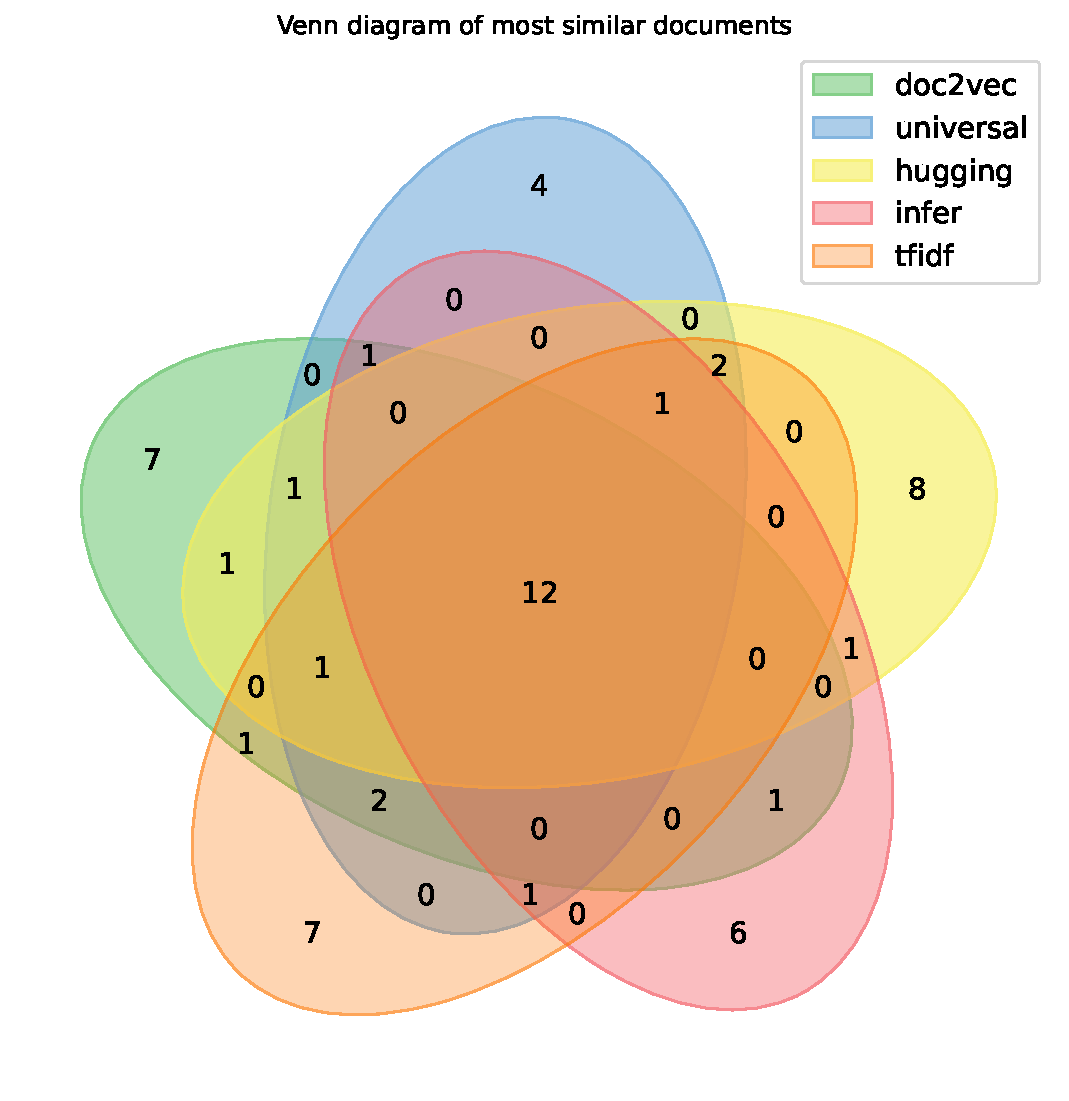
\includegraphics[width=4cm]{images/comparison/Venn_diagram_of_most_similar_documents.pdf} }}%
    \qquad
    \subfloat[\centering Heatmap visualizing shared query results.]{{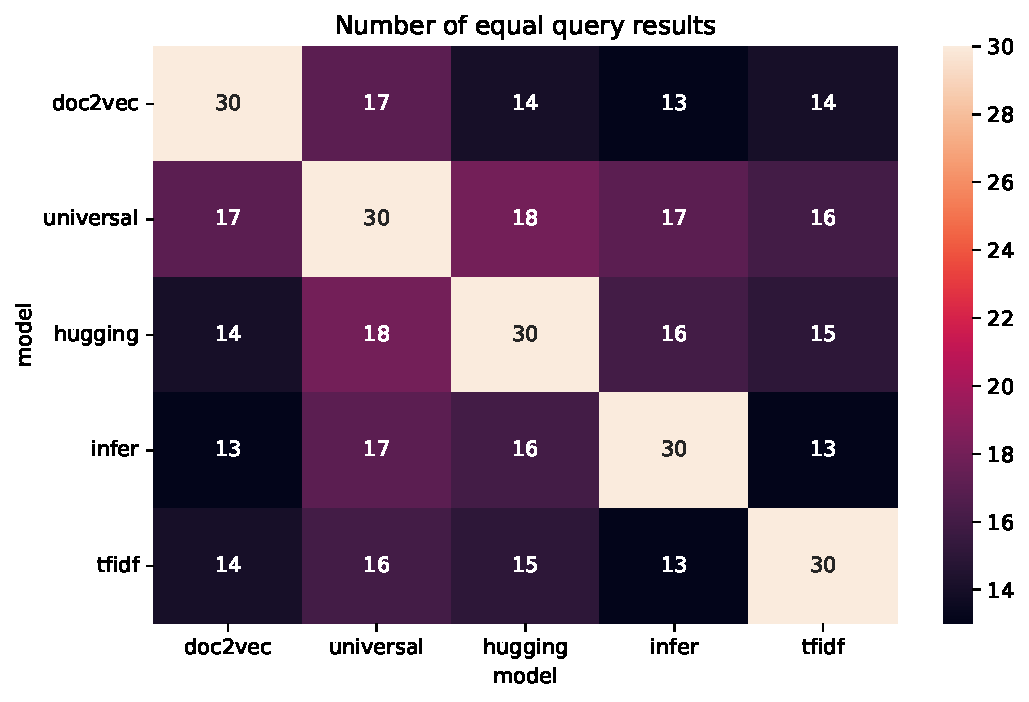
\includegraphics[width=6cm]{images/comparison/Number_of_equal_query_results.pdf} }}%
    \caption[Comparison of models]{Comparison of the results obtained by different models.}%
    \label{fig:comparison-models}%
\end{figure}


% sample query
To display the differences between the models exemplary, the five most similar documents to a random document were returned from the database and visualized.
The text of the query document was encoded using the respective model and a 
\ac{knn} query was used to obtain the results from the local database containing 2048 documents.
The query image, i.e. the one surrounded with a border, was omitted from the database query response.
The query responses are listed according to descending similarity to the query document.
\autoref{fig:query_resp_doc2vec} displays the \ac{d2v} reponses,  
\autoref{fig:query_resp_sbert} displays the \ac{sbert} reponses,  
\autoref{fig:query_resp_tfidf} displays the \ac{tfidf} reponses,  
\autoref{fig:query_resp_infer} displays the \infersent{} reponses,  
\autoref{fig:query_resp_use} displays the \ac{use} reponses.

All models except \ac{d2v} and \ac{use} returned only documents of \textit{CREDIT SUISSE}.
Apart from this difference, the query responses of the models are very similar.


% sample query
\begin{figure}[h!]
    \begin{subfigure}{\textwidth}
        \centering
        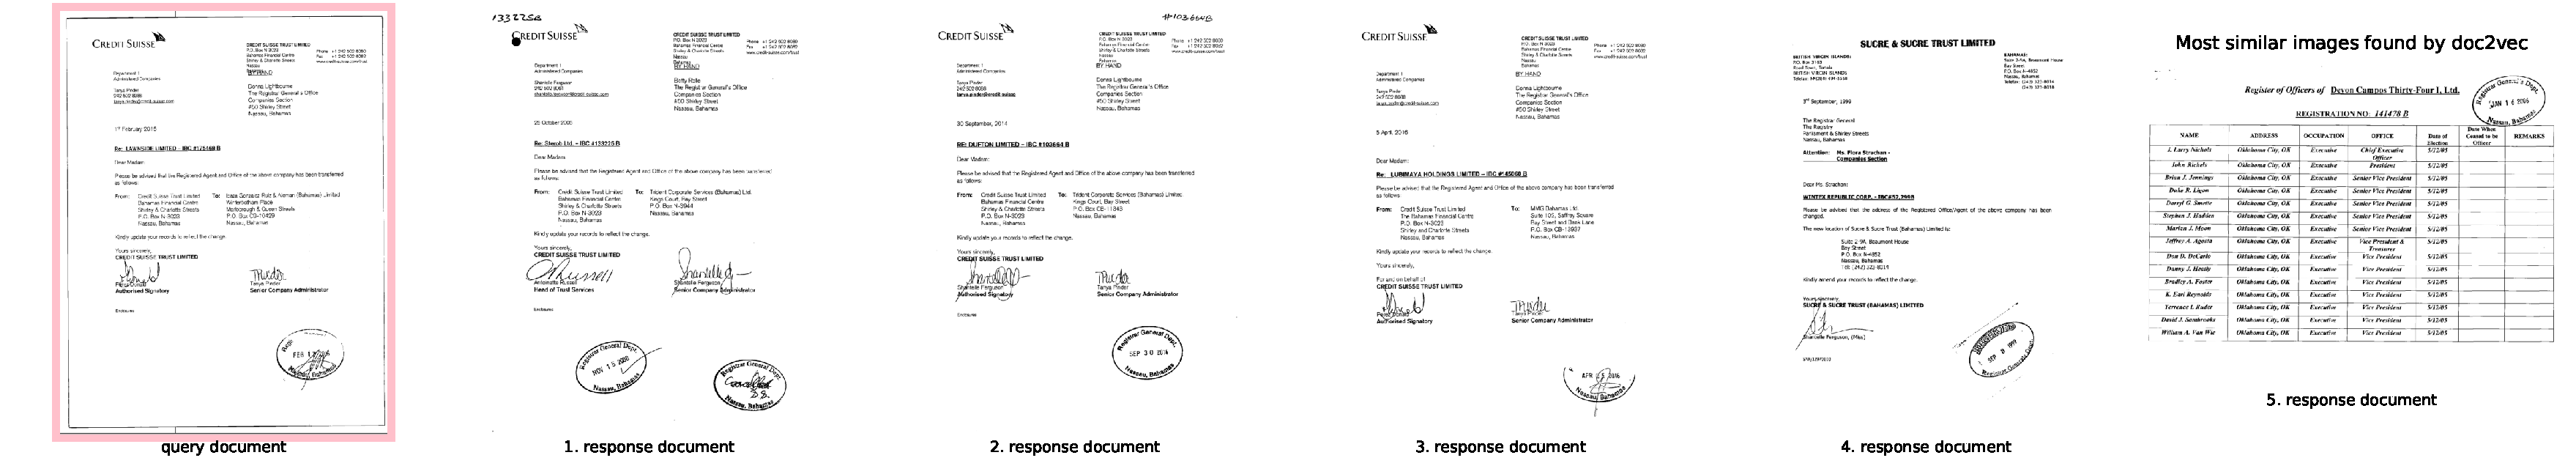
\includegraphics[width=1\textwidth]{images/query_results/4b4d0a9ee0c7283e5bfd69c402c73b2140bf90351c8f44d6809afe23c6dfaa50/Most_similar_images_found_by_doc2vec.pdf}
        \caption{\ac{d2v}}
        \label{fig:query_resp_doc2vec}
    \end{subfigure}

    \begin{subfigure}{\textwidth}
        \centering
        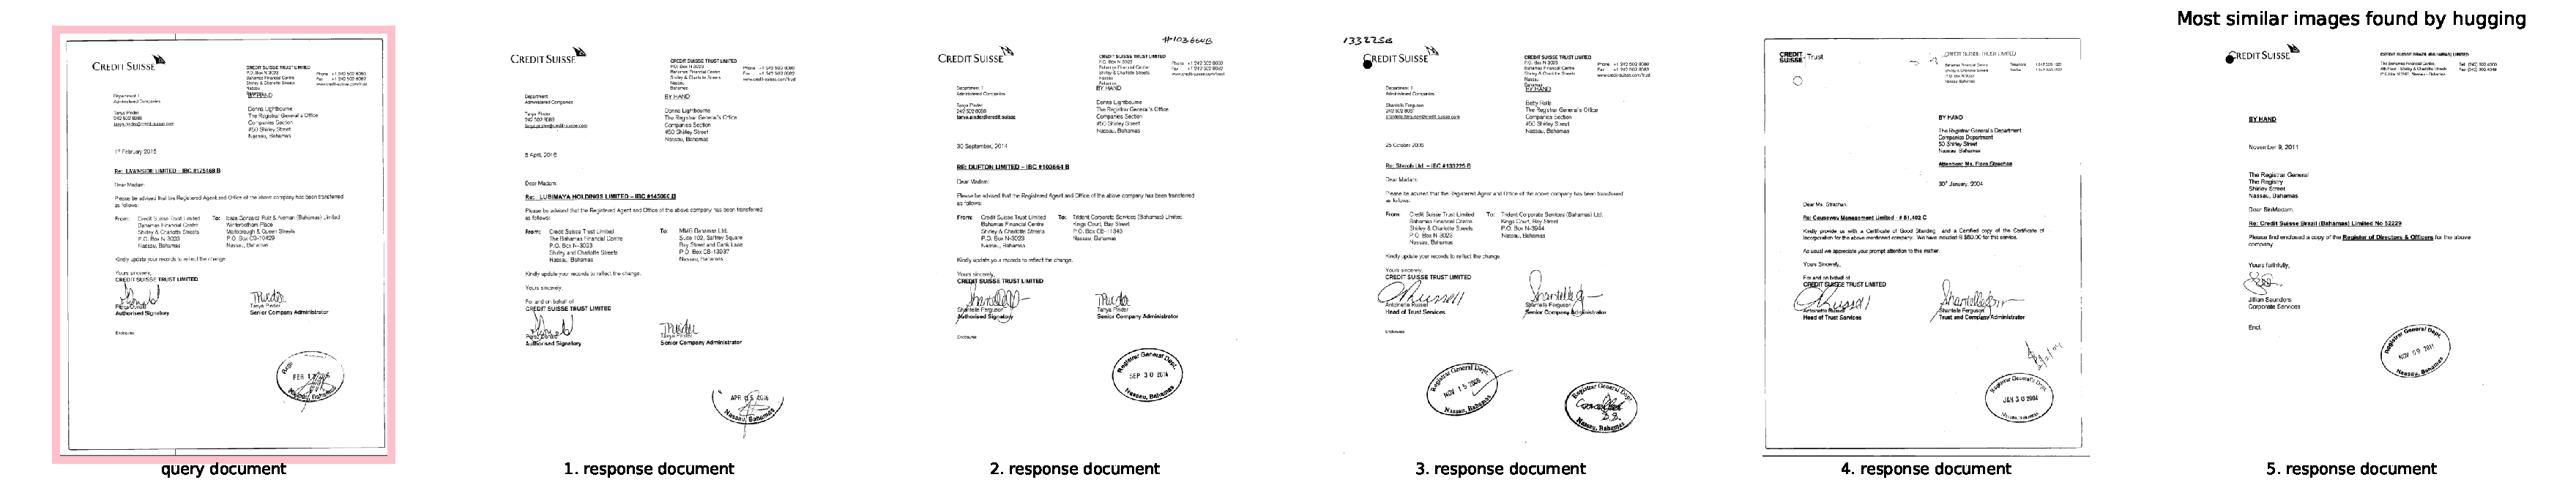
\includegraphics[width=1\textwidth]{images/query_results/4b4d0a9ee0c7283e5bfd69c402c73b2140bf90351c8f44d6809afe23c6dfaa50/Most_similar_images_found_by_hugging.pdf}
        \caption{\ac{sbert}}
        \label{fig:query_resp_sbert}
    \end{subfigure}

    \begin{subfigure}{\textwidth}
        \centering
        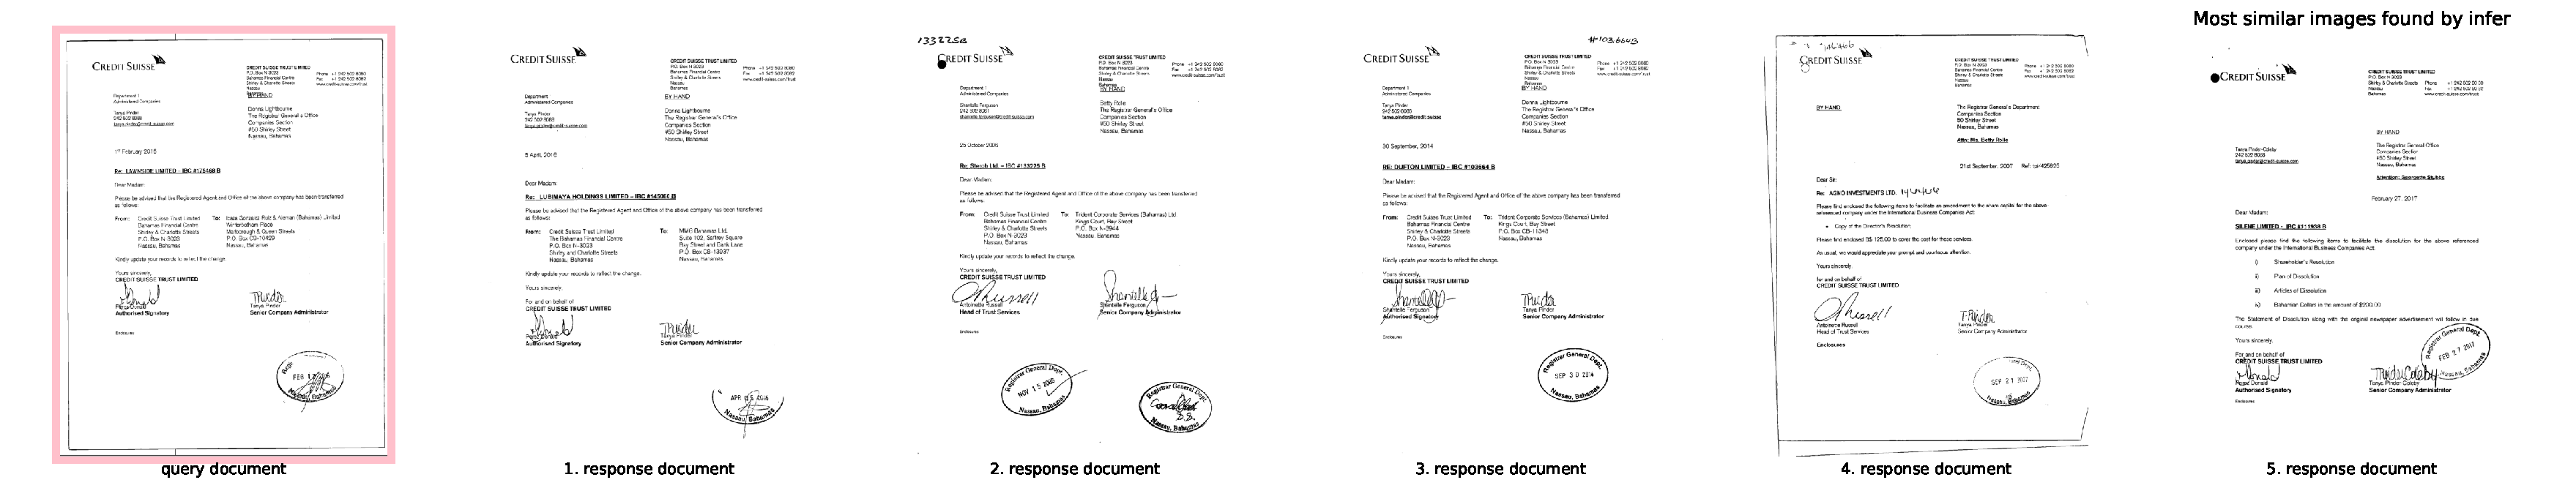
\includegraphics[width=1\textwidth]{images/query_results/4b4d0a9ee0c7283e5bfd69c402c73b2140bf90351c8f44d6809afe23c6dfaa50/Most_similar_images_found_by_infer.pdf}
        \caption{\infersent{}}
        \label{fig:query_resp_infer}
    \end{subfigure}

    \begin{subfigure}{\textwidth}
        \centering
        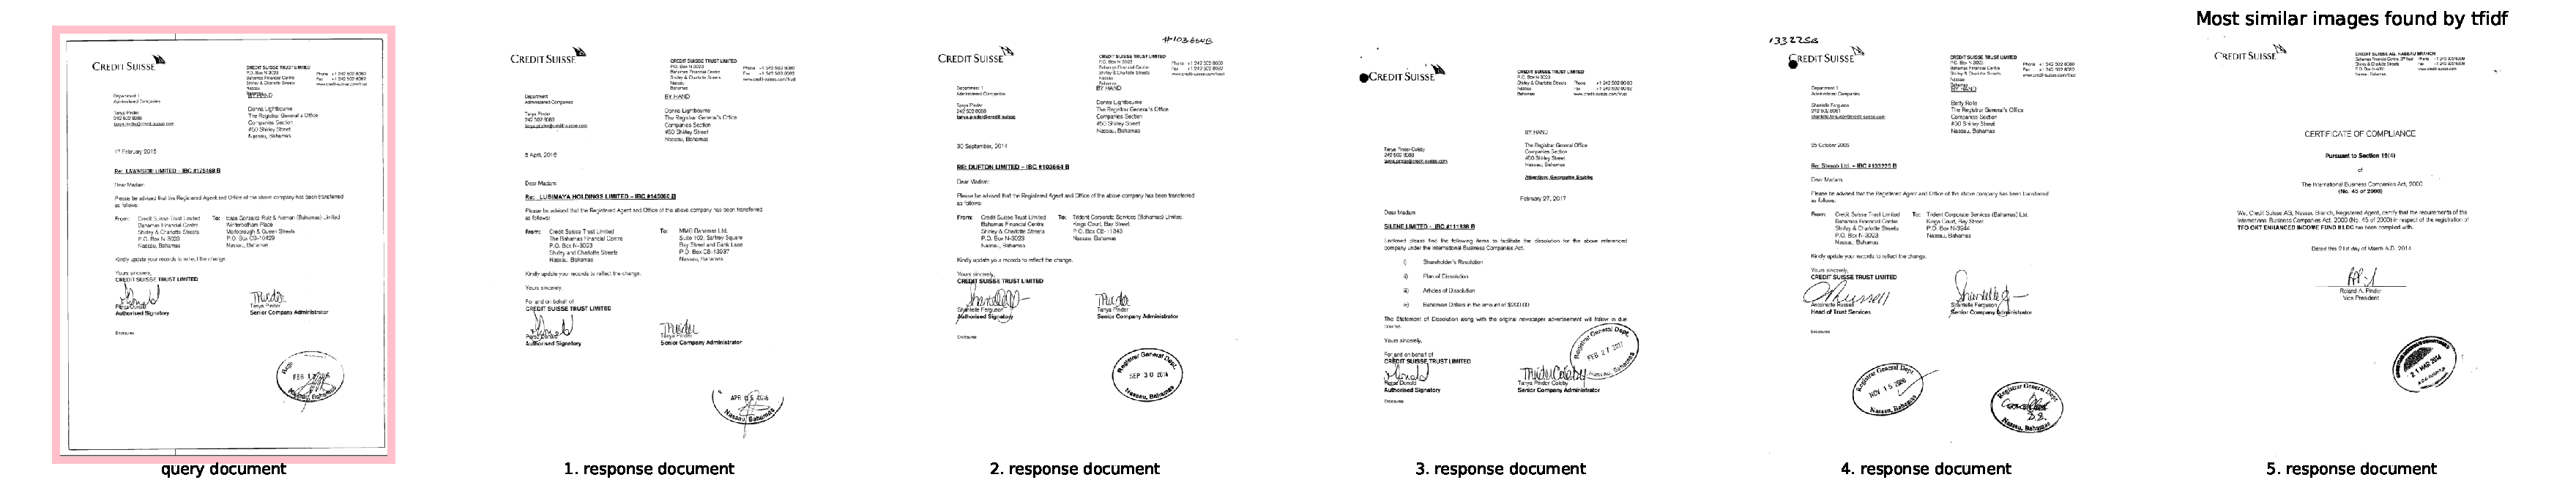
\includegraphics[width=1\textwidth]{images/query_results/4b4d0a9ee0c7283e5bfd69c402c73b2140bf90351c8f44d6809afe23c6dfaa50/Most_similar_images_found_by_tfidf.pdf}
        \caption{\ac{tfidf}}
        \label{fig:query_resp_tfidf}
    \end{subfigure}

    \begin{subfigure}{\textwidth}
        \centering
        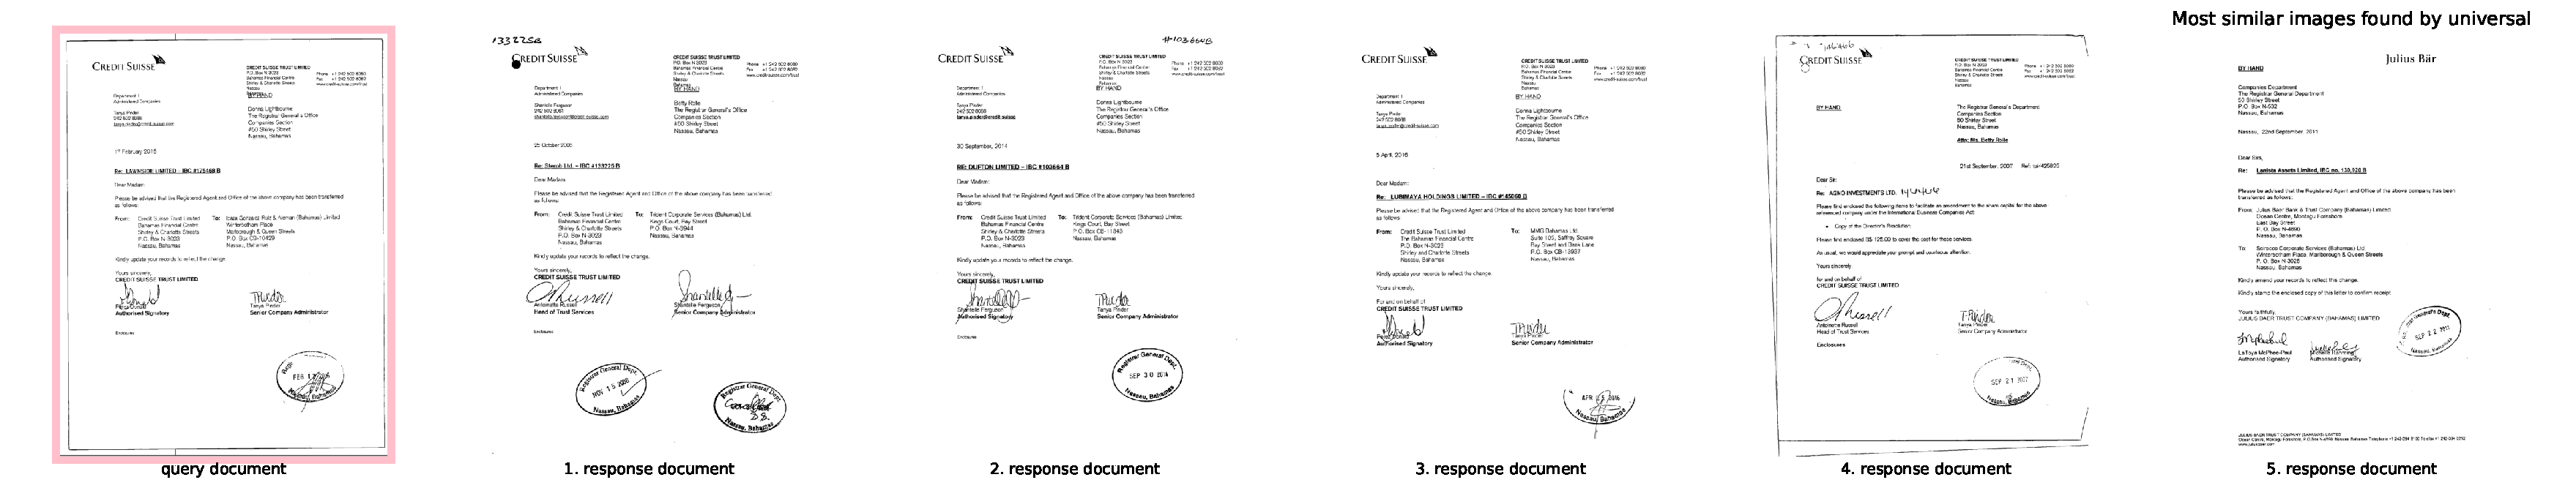
\includegraphics[width=1\textwidth]{images/query_results/4b4d0a9ee0c7283e5bfd69c402c73b2140bf90351c8f44d6809afe23c6dfaa50/Most_similar_images_found_by_universal.pdf}
        \caption{\ac{use}}
        \label{fig:query_resp_use}
    \end{subfigure}
\caption[Exemplary query response]{Response of exemplary query in terms of similarity on different embeddings.}
\label{fig:query_resp}
\end{figure}

% good results
The models produced good query responses on a query document consisting of little text.
A sample query document is shown in \autoref{fig:good_query_resp_infer}.
Even though at first glimpse, the response documents seem to appear unrelated to the query document, they share multiple words, such as \textit{director}.
Similar response documents do not have to of similar visual appreance results from the fact that the text embeddings only consider information from the text layer.

\begin{figure}[htp] % htp = hier (h), top (t), oder auf einer eigenen Seite (p).
    \centering
    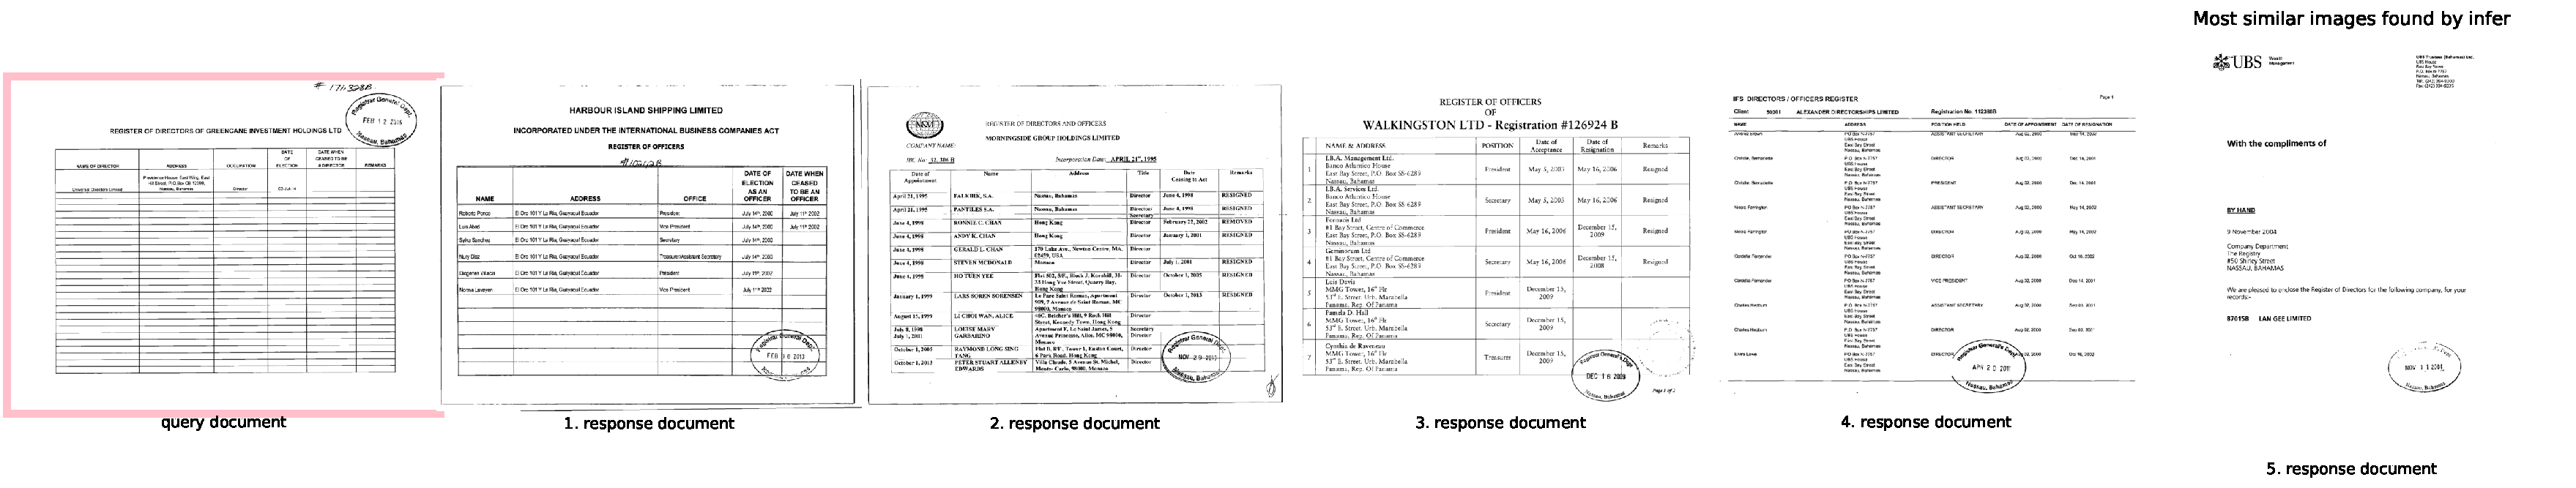
\includegraphics[width=1\textwidth]{images/query_results/42b7e56855c88c22ed01f381167e6f0887815e1ef7ea6b149be06ee1f8557b9e/Most_similar_images_found_by_infer.pdf}
    \caption[\infersent{} query responses]{\infersent{} query responses on a query document consisting of little text.
    }
    \label{fig:good_query_resp_infer}
\end{figure}

% bad results
\textcolor{red}{TODO}
\begin{figure}[h!]
    \ContinuedFloat
    \begin{subfigure}{\textwidth}
        \centering
        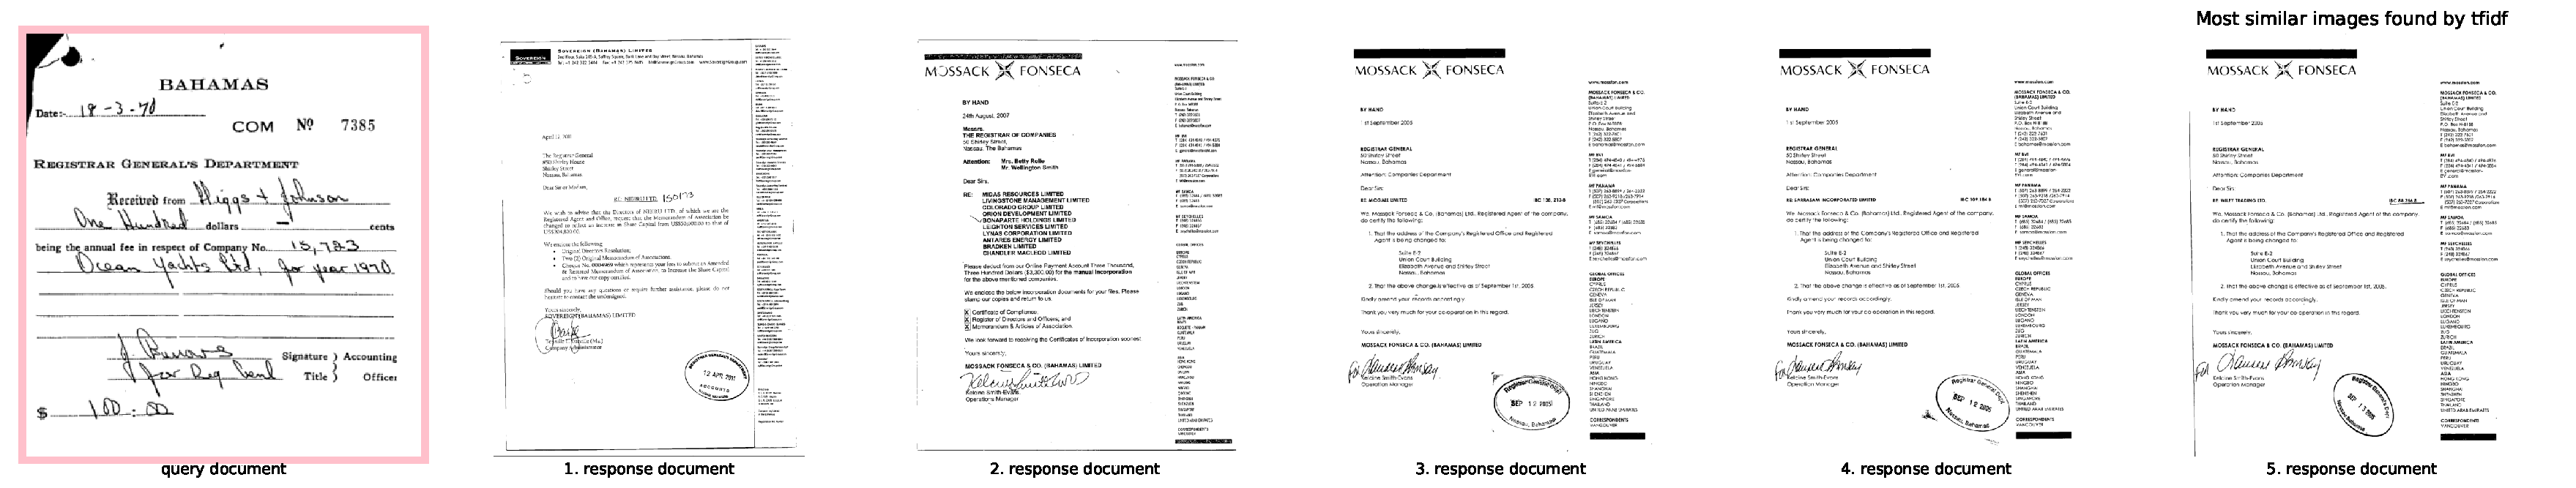
\includegraphics[width=1\textwidth]{images/query_results/4542b223317eba23e4bda3e1536d61c8e2d2890a6439830ca8c62650bc1aac70/Most_similar_images_found_by_tfidf.pdf}
        \caption{\ac{tfidf}}
        \label{fig:bas_query_resp_tfidf}
    \end{subfigure}

    \begin{subfigure}{\textwidth}
        \centering
        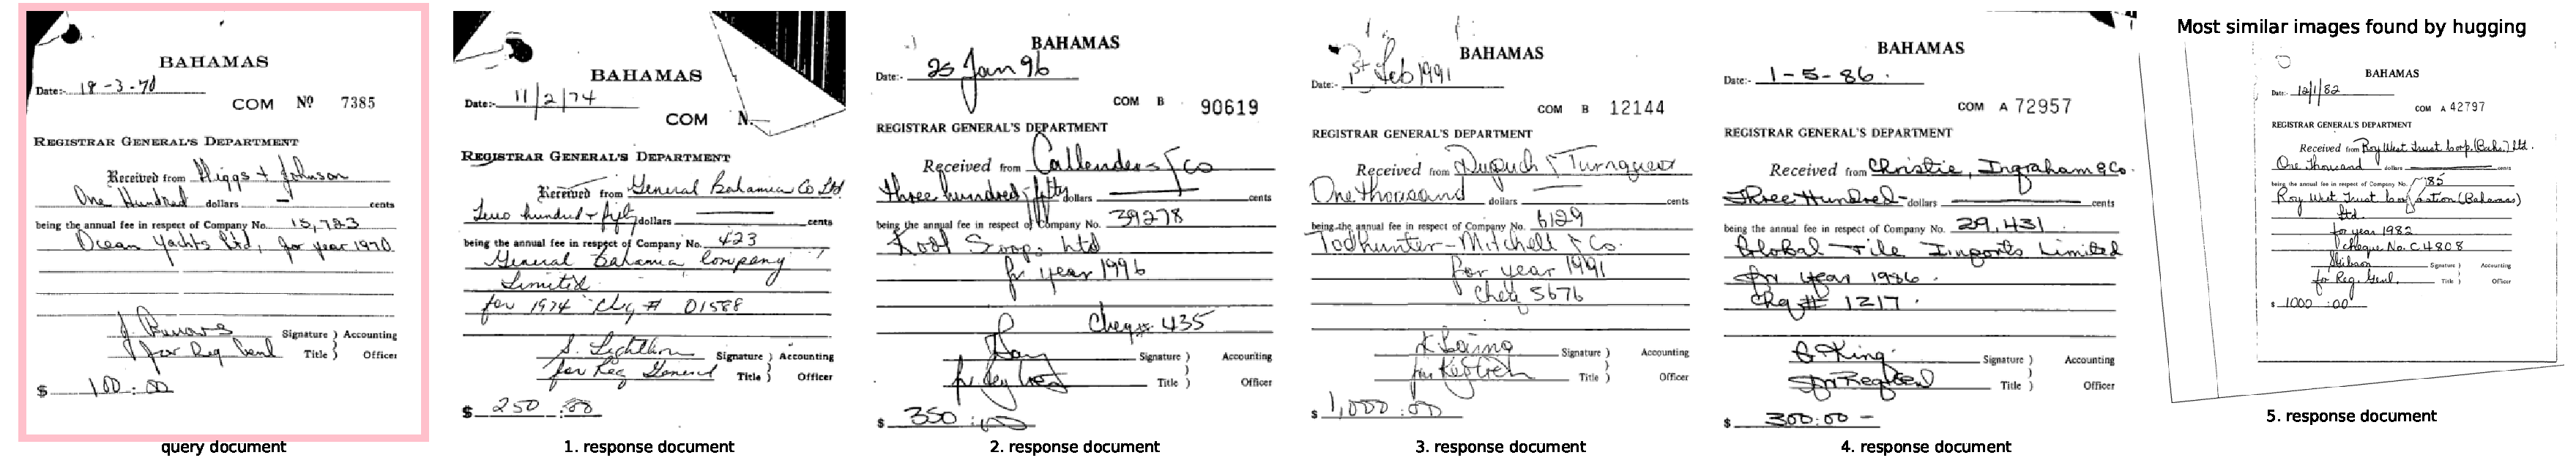
\includegraphics[width=1\textwidth]{images/query_results/4542b223317eba23e4bda3e1536d61c8e2d2890a6439830ca8c62650bc1aac70/Most_similar_images_found_by_hugging.pdf}
        \caption{\ac{sbert}}
        \label{fig:good_query_resp_sbert}
    \end{subfigure}

\caption[Qualitative comparison of query responses]{Qualitative comparison of query responses.
The majority of the query document consists of handwritten text.
The results of the \ac{tfidf} model are not very similar to the query document and thus, are considered to be of poor quality.
The other models, for example \ac{sbert}, produce results which are more similar to the query document.
}
\label{fig:comp_query_resp}
\end{figure}



% investigate certain images
any images which produce unusual results?

\section{Comparison with baseline topic analysis approach}\label{sec:evaluation-top-model-app}

The baseline topic analysis \ac{t2v} offers a variety of built-in functionalities to the user.
It is possible to retrieve human interpretable inherent topics of a set of documents, 
as well as the topics most similar to certain search terms 
and \wordcloud{}s of these results.
Hence, this library meets the needs articulated by this work.

% > 1 embedding model
Opposed to \ac{t2v}, this thesis proposes a composite of different approaches to encoding visual and semantic information 
and query for them using a database and visualization by the means of \wordcloud{}s.
To be more specific, this thesis not only relies on one semantic embedding model but offers several techniques and an approach to incorporate visual information.

% no topics for search terms
However, it is not possible to query for topics of the corpus which best describe a search term.
Alternatively, one can perform a fuzzy text search on the documents.
The user can inspect the \ac{pdf} of a document upon clicking on its name in the list of documents.
The detail component enables the investigation of similar documents in terms of different embedding approaches.

% topic definition
Due to \ac{t2v}'s architecture, documents and words are mapped into the same \ac{vsm}.
Hence, the topic vector definition and representation by its closest words are more meaningful than the approach of the thesis. 
In this thesis, a topic is represented by frequent words in the set of documents that are not necessarily meaningful. 

% term frequency
The tool implemented in this thesis can display the term frequency of the document chosen in the detail component.
The \ac{t2v} library does not offer a comparable service.